\documentclass[12pt]{article}
\usepackage{amsfonts}
\usepackage{amsmath}
\usepackage{amssymb}
\usepackage[parfill]{parskip}
\usepackage{amsthm}
\usepackage{hyperref}
\usepackage{graphicx}
\usepackage{tikz}
\usetikzlibrary{automata, positioning} %for state diagrams


\graphicspath{{./images/}}

\hypersetup{
    colorlinks=true,
    linkcolor=blue,
    filecolor=magenta,
    urlcolor=cyan,
}

\theoremstyle{definition}
\newtheorem{definition}{Definition}[section]
\newtheorem{theorem}{Theorem}[section]
\newtheorem{corollary}{Corollary}[theorem]
\newtheorem{lemma}[theorem]{Lemma}
\newtheorem{proposition}{Proposition}[section]
\newtheorem{example}{Example}[section]




\begin{document}

\title{Stochastic Processes}
\author{Riley Wilson}
\date{last updated: 1/4/2021}
\maketitle

These are notes compiled when I took math 171 at UCLA as taught by Moritz Voss. The textbook used for the course was Durrett's \textit{Essentials of Stochastic Processes},\footnote{The text is freely available online if your organization has access to Springer Books.} so what follows is bound to be similar.

The document is arranged by week and lecture number, not mathematical content. Some weeks only have two lectures since there was a holiday or I decided to compress two classes' worth of material under one heading. Occasionally, I include material covered during discussion section. You'll find these notes titled "Jacob's section."

Any mathematical mistakes/typos are my own.

\section{Week 0}

First, we must understand what we mean by "stochastic". "Stochastic" in our context is very close in meaning to "random" For our purposes, imagine they are interchangeable.

Mathematically, we define something called a stochastic process.

\begin{definition}{\textbf{Stochastic Process}}
  A stochastic process is a collection of random variables $(X_t)$ $t \in I$, where $I$ is the index set of the process. The random variables are defined on a common scenario space, $\Omega$ and take values in a common state space, $S$. Formally, we say

\begin{align*}
  &X_t: \Omega \rightarrow S,
  &\omega \mapsto X_t(\omega) = x \in S
\end{align*}

Remember, if $S \subseteq \mathbb{N}$, we say $X_t$ is a discrete random variable process. Likewise, if $S \subseteq \mathbb{R}$, it would be a continuous one. We will get to continuous-time stochastic processes later in the notes.
  \end{definition}

Why are stochastic processes important? Let's consider a problem where they can be helpful.

\textbf{Gambler's Ruin problem}: Suppose we go to the casino with 10 dollars and need 80. We play european-style roulette, betting 1 dollar on red each time. If we win, we get our 1 dollar back, plus an extra dollar. If we lose, we lose the dollar. The probability of getting red on any given spin is $p = \frac{18}{37} \approx .486$. What is the probability we go bankrupt (are 'ruined') before winning 80 dollars?

\textbf{Solution}: First, we consult our intuition to get a sense of the problem. We know the game is "unfair", as the probability of winning a bet is below .5. But is it mathematically unfair? What's the expected value?

Let $W = P -c$ where $P$ is a random variable representing our payout and c is our stake, or what we originally bet.

\begin{align*}
  \mathbb{E}[W] = \mathbb{E}[P] - c &= 2c(p) + 0(1-p) -c \\
   &= c(2p -1)  = \frac{-c}{37} < 0
\end{align*}

Which is not unfair.

To simplify things, we can model red with a random variable, $X_i$. $P(X_i =1) = p$, and $P(X_i = -1) = 1-p$.

We can define the gambler's total wealth as $S_n$, where $n$ is the number of times she's made a bet. Hence, $S_0 = 10$, and

$$
S_n = S_0 + X_1 + X_2 +\dots + X_n = S_0 + \sum_{i=1}^n X_i
$$

Where $n \geq 1$. Recall definition 1.1 and see $S_n$ is a stochastic process. We introduce a new concept to sharpen our thinking about the problem.


\begin{definition}{\textbf{Hitting times}}
A "hitting time" is a random variable whose observed value is the time a stochastic process reaches a specific value.

For the gambler's ruin problem, we'll define hitting times as:

\begin{align*}
  &T_0 = \text{min}\{n \geq 1: S_n = 0\} &T_{80} = \text{min}\{ n \geq: S_n = 80\}
\end{align*}

\end{definition}

Note $T_0$ and $T_{80}$ are random variables that tell us when the gambler goes bankrupt or wins. In this vocabulary, we can describe the ruin probability as:

$$
P(T_0 < T_{80})
$$

We could immediately calculate this if we knew the joint probability distribution of $T_0$ and $T_{80}$. Unfortunately, we don't.

A different way relies on defining a "ruin function." Say

$$
B_k = \{\text{gambler goes bankrupt with k initial capital before reaching K}\}
$$

The ruin function is $R(k) = P(B_k)$. Notice $R(0) = 1$ and $R(K) = 0$.

We then introduce an event set.

$$
W = \{\text{gambler wins first round}\}
$$

Now, we can examine the ruin function a little closer.

\begin{align*}
  R(k) &= P(B_k) \\
  &= P(B_k \mid W)P(W) + P(B_k \mid W^c)P(W^c) \\
  &\text{(by the law of total probability)} \\
  & = P(B_{k+1})P(W) + P(B_{k-1})P(W^c)
\end{align*}

The last step is justified by the Markov property of a random walk. We will cover this later.

We can get a recursive formula for $R(k)$ this way.

\begin{align*}
  R(k) &= R(k+1)P(W) + R(k-1) P(W^c) \\
  &= R(k+1)(p) + R(k-1)(1-p)
\end{align*}


We can solve this and get a closed form. The method is a little lengthy, and involves iterating the difference equation and a telescoping series. The calculations are not conceptually important. In the end, we get:

\begin{align*}
  R(k) = \frac{(\frac{1-p}{p})^k - (\frac{1-p}{p})^K}{1- (\frac{1-p}{p})^K}
\end{align*}

for all $k = 1, \dots, K$. Now, we can get the ruin probability for different starting capitals ($k$), target capitals ($K$), and probabilities of winning ($p$). For instance, if $k =10$, $K = 80$, and $p = .486$, then

\begin{align*}
  R(10) = \frac{(\frac{.514}{.486})^{10} - (\frac{.514}{.486})^{80}}{1- (\frac{.514}{.486})^{80}} = .9914
\end{align*}

In words, our gambler is going to have a bad time.

We've solved the problem, but we might want to see what happens if the gambler changes her strategy. For instance, she might bet 2 dollars each time instead of 1. What is the ruin probability then?

Our current closed form works perfectly for this. Imagine each "dollar" is now a chip, with $x$ dollars. Now, the gambler bets $x$ dollars, or 1 chip, per round. As before, she loses all the money if she loses the round, and wins it back at 1:1 odds if she wins. $p$ doesn't need to be modified on the new interpretation. The new $k$ and $K$'s only need to be divided by $x$.

The ruin probability if the gambler bets 5 dollars per round is:

\begin{align*}
  R(10/5) &= \frac{(\frac{.514}{.486})^{10/5} - (\frac{.514}{.486})^{80/5}}{1- (\frac{.514}{.486})^{80/5}} \\
  & = \frac{(\frac{.514}{.486})^{2} - (\frac{.514}{.486})^{16}}{1- (\frac{.514}{.486})^{16}} \\
  & = .9182
\end{align*}

She does better. As it turns out, because this is a negative expected value game the optimal strategy is to minimize the number of bets you need to reach $K$. This means you should go all in every time.

The best ruin probability is then:
\begin{align*}
  1-P(\text{reaching 80}) = 1-(.486)^3 = .8852.
\end{align*}

\subsection{bonus: computation}
There's another way to compute the ruin probability given different initial starting capitals and targets. It's possible to simulate the gambler's game with some simple code. If you run the simulation many times, you can count how many times the gambler "won" and reached the target amount, and "lost," or was ruined. The ratio of these two numbers will be an approximation of the ruin probability.

A graph of 100 possible "paths" a gambler's wealth can take is shown below.\footnote{The graph was generated from code supplied by Moritz Voss. Notice how some paths are very long. This might give the gambler the impression she has a chance, even though her probability of reaching the target amount is actually very low. I imagine casinos like this property of the game.} As in our problem, the gambler starts with 10 dollars and stops if she reaches 80 dollars.

\begin{center}
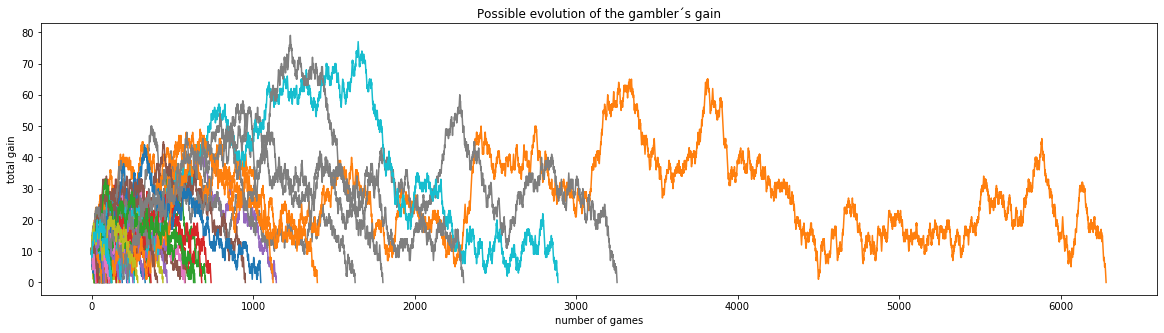
\includegraphics[scale = .35]{index.png}
\end{center}

I will not reproduce the code. It only takes a little python to replicate.


\section{Week 1}
\subsection{Lec 1 and 2}


\begin{definition}{\textbf{Markov Chain}}
Let $S$ be a discrete set. A Markov chain is a sequence of random variables, $X_0, X_1, X_2, \dots$ takings values in $S$ with the property:

\begin{align*}
  &P(X_{n+1} = j \mid X_0 = i_0, X_1 = i_1 \dots X_{n} = i_n) \\
  &= P(X_{n+1} = j \mid X_n = i)
\end{align*}

For all $i_0 \dots i_{n-1}$ in $S$ and $n \geq 0$. $S$ is the state space of the Markov chain.

\end{definition}

In words, this means the next random variable is influenced only by the previous one. If we are given a Markov chain and asked to compute the value of $X_{100}$, for instance, we only need to know the value of $X_{99}$.

A concrete example helps. Imagine a sequence of random variables represents my mood on a given day. If the sequence is a Markov chain, my mood on day 100 is only influenced by my mood on day 99.



\begin{definition}{\textbf{Time Homogeneous Markov Chain}}
A time homogeneous Markov chain is one where:
\begin{align*}
  P(X_{n+1} = j \mid X_n = i) = P(X_1 = j \mid X_0 = i)
\end{align*}

For all $i,j \in S$ and $n\geq 0$.
\end{definition}

\theoremstyle{definition}
\begin{definition}{\textbf{Transition Probability Matrix}}
We define a transition probability matrix as $P = (P_{i,j})$, $i,j \in S$ where
\begin{align*}
  P_{i,j}= P(X_1 = j \mid X_0 = i)
\end{align*}


\begin{example}[Weather model]
Let $(X_n)$, $n \geq 0$ be a time homogeneous Markov chain with state space $S = \{1,2,3\}$ where $1= \text{rainy}, 2 = \text{sunny}, 3 = \text{cloudy}$. $X_n$ corresponds to the weather on day $n$.

We define a transition probability matrix:

\begin{align*}
  P =
  \begin{bmatrix}
  .2 & .6 & .2 \\
  .1 & .8 & .1 \\
  .1 & .6 & .3 \\
\end{bmatrix}
\end{align*}

The $i,j$th entry gives us the transition probability of moving to $j$ given $i$. All the entries are condition probabilities. In light of this, the fact all the rows sum to $1$ is unsurprising.

We can represent the transition probability matrix with a Markov chain diagram.

\begin{center}
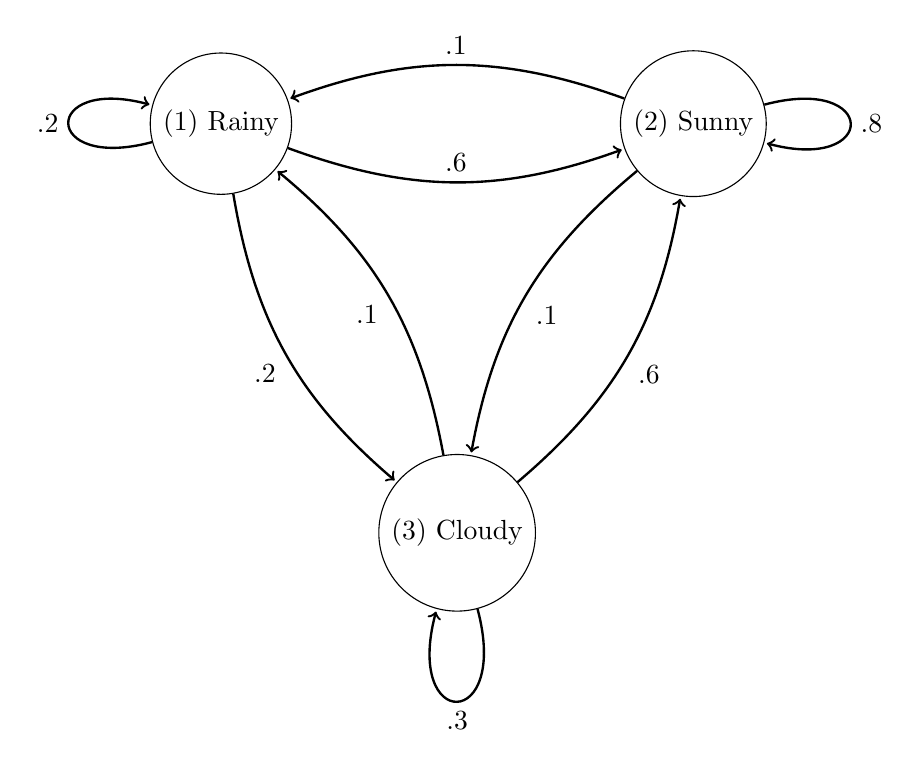
\begin{tikzpicture}



        % Draw the states
        \node[state] at (0, 0)     (rainy)     {(1) Rainy};
        \node[state] at (6, 0)     (sunny)     {(2) Sunny};
        \node[state] at (3, -5.196) (cloudy) {(3) Cloudy};

        % Connect the states with arrows
        \draw[every loop,
              auto=right,
              line width=.3mm,]
            (rainy)     edge[bend right=20]            node {.2} (cloudy)
            (rainy)     edge[bend right=20, auto=left] node {.6} (sunny)
            (sunny)     edge[bend right=20]            node {.1} (rainy)
            (sunny)     edge[bend right=20, auto=left] node {.1} (cloudy)
            (cloudy) edge[bend right=20]            node {.6} (sunny)
            (cloudy) edge[bend right=20, auto=left] node {.1} (rainy)
            (rainy) edge[loop left] node {.2} (rainy)
            (cloudy) edge[loop below] node {.3} (cloudy)
            (sunny) edge[loop right] node {.8} (sunny);
    \end{tikzpicture}


\end{center}

Each edge is labeled with the probability we transition from one state to another. Loops are labeled with the probability we stay in the same state.

\end{example}

\end{definition}


\begin{definition}{\textbf{Stochastic Matrix}}
  A stochastic matrix is a square matrix, $P = P_{i,j}$, $i,j \in S$ which satisfies:
  \begin{enumerate}
    \item $ 0 \leq P_{i,j} \leq 1,$ $\forall i,j$.
    \item $\sum_{j \in S} P_{i,j} = 1$, $\forall i$.
  \end{enumerate}
\end{definition}

If we have a matrix that describes our transition probabilities, what about our initial distribution? How do we know what we are transitioning from?


\begin{definition}{\textbf{Transition Vector}}
  Let $(X_n)$, $ n = 0,1, \dots$ be a Markov chain. The distribution of $X_0$ is the initial distribution of the entire chain. $X_0$'s distribution is written as:

  \begin{align*}
    \alpha^T = (\alpha_1, \alpha_2, \alpha_3 \dots)
  \end{align*}

  Where $P(X_0 = i) = \alpha_i$. We might also call $\alpha$ a probability vector, since $ 0 \leq \alpha_i \leq 1$ $\forall i$ and $\sum_{i \in S} \alpha_i = 1$.
\end{definition}

\subsection{Lec 3}


\begin{example}{Weather Model Computation}
  What is $P(X_2 = 3 \mid X_0 = 2)$?

  We rewrite in terms of one-step probabilities.

  \begin{align*}
    P(X_2 = 3 \mid X_0 = 2) &= \sum_{k \in S}P(X_2 = 3, X_1 = k \mid  X_0 = 2) \text{(by LTP)} \\
    &=\sum_{k \in S} \frac{P(X_2 = 3, X_1 = k, X_0 = 2)}{P(X_0 = 2)} \\
    &=\sum_{k \in S} \frac{P(X_2 = 3, X_1 = k, X_0 = 2)}{P(X_0 = 2)} * \frac{P(X_1 = k, X_0 = 2)}{P(X_1 = k, X_0 = 2)} \\
    &=\sum_{k \in S} \frac{P(X_2 = 3, X_1 = k, X_0 = 2)}{P(X_1 = k, X_0 =2)} \frac{P(X_1 = k, X_0 = 2)}{P(X_0 = 2)} \\
    &= \sum_{k \in S} P(X_2 = 3 \mid X_1 = k, X_0 =2) P(X_1 = k \mid X_0 = 2) \\
    &= \sum_{k \in S} P(X_2 = 3 \mid X_1 = k) P(X_1 = k \mid X_0 = 2) \\
    &\text{we ignore $X_0 = 2$ by the Markov property} \\
    &= \sum_{k \in S} P_{k,3}P_{2,k} = P_{2,3}^2
  \end{align*}
\end{example}



\begin{example}{Joint Probabilities}
  There's a multiplication rule for the probability of a certain sequence in a time-homogeneous Markov chain. Let $i,j,k \in S$.

  \begin{align*}
    P(X_1=i, X_2=j, X_3=k) &= P(X_1=i)P(X_2 = j \mid X_1 = i)P(X_3=k \mid X_1 = i, X_2 = j) \\
    &= P(X_1 = i)P_{i,j}P_{j,k} \\
    \intertext{Note that $P(X_1 = i) = \sum_{m \in S} P(X_1 =i \mid X_0 = m) = (\alpha^T P)_i$. Substituting, we get:}
    &=(\alpha^T P)_i P_{i,j}P_{j,k}
  \end{align*}
\end{example}



\begin{proposition}{\textbf{Chapman-Kolmogorov equation}}
  Let $(X_n)$ be a stochastic process and $i,j,k \in S$. Then,
  \begin{align*}
    P(X_{n+m} = j \mid X_0 = i) &= \sum_{k \in S}P(X_m = k \mid X_0 = i)P(X_n = j \mid X_0 = k) \\
    &\iff P_{i,j}^{n+m} = \sum_{k \in S} P_{i,k}^mP_{k,j}^n \\
    &\iff P^{n+m} = P^nP^m
  \end{align*}
\end{proposition}

(We will explore the proof to this later. Also, take a look at the last line. Check how it relates to the second to last line.)


\begin{definition}{Marginal distribution}
  Notice for all $n \geq 1$,

  \begin{align*}
    P_{\alpha}(X_n = j) &= \sum_iP_{\alpha}(X_n = j \mid X_0 = i)P_{\alpha}(X_0 = i) \\
    &= \sum_i \alpha_i^T (P^n)_{i,j} = (\alpha^T P^n)_j
  \end{align*}

Then, we say the marginal distribution of $X_n$ is
\begin{align*}
  \mu_{X_n}^T = \alpha^TP^n & \text{where} & (\mu_{X_n})_j = P_{\alpha}(X_n = j)&
\end{align*}

\end{definition}


\begin{definition}{\textbf{Joint Distributions}}
  Let $(X_n)$ be a time homogeneous Markov chain. For all $k \in \mathbb{N},$ $0 \leq n_1 \leq \dots \leq n_k$, and all states $i_1, \dots \in S$,

  \begin{align*}
    P_{\alpha}(X_{n_1} = i_1, X_{n_2} = i_2 \dots X_{n_k} = i_k) = (\alpha^TP^{n_1})_{i_1}(P^{n_2 - n_1})_{i_1, i_2} \dots  (P^{n_k - n_{k-1}})_{i_{k-1}, i_k}
  \end{align*}

Hence, $P$ and $\alpha$ completely determine a Markov chain.
\end{definition}

\section{Week 2}
\subsection{Lec 1}


\begin{theorem}{Markov property (different statement):}
  For all $m< n$,

  \begin{align*}
    &P(X_{n+1} = j \mid X_0 = i_0, \dots X_{n-m} = i) \\
    &= P(X_{n+1} = j \mid X_{n-m} = i) \\
    &= P(X_{m+1} = j \mid X_0 = i) = (P^{m+1})_{i,j}
  \end{align*}

  for all $i,j, i_0 \dots i_{n-m-1}$.
\end{theorem}

We want to classify the states of a Markov chain. First, we introduce some notation. Let,

\begin{align*}
  P_x(X_n = j) = P(X_n = j \mid X_0 = x)
\end{align*}

Also, recall an identity for conditional expectation:

\begin{align*}
  \mathbb{E}[X_n \mid X_0 = x] &= \sum_{k \in S} k P(X_n = k \mid X_0 = x) \\
  &= \sum_{k \in S} k P_{x,k}^n
\end{align*}


\begin{definition}[\textbf{Return Times}]
  Given a Markov chain $(X_n)_{n = 0,1...}$ let $T_y = \text{min}\{n \geq 1: X_n = y\}$ be the time of the first return to states $y \in s$. If $X_n \ne y $ for all $n \geq 1$, set $T_y = + \infty$.
\end{definition}

We can do more with this notion of return times.

Let $\rho_{yy} = P_y(T_y < \infty)$ be the return probability. In words, it is the probability we return to state $y$ after starting at $y$. Likewise, $\rho_{xy} = P_x(T_y < \infty)$ is the probability we go from $x$ to $y$ in a finite number of steps.


\begin{definition}[\textbf{Stopping times}]
  We say a random variable $T$ is a stopping time with respect to a Markov chain $(X_n)_{n = 0,1 \dots}$ if for each $n \geq 0$ the occurrence of $\{T = n\}$ can be determined by the values of the process $X_0, X_1, \dots X_n$ up to time $n$.
\end{definition}

In words, we can't 'look into the future' to determine if our random variable takes on a value or not.


 \begin{example}
   Let $T_y = \text{min}\{n \geq 1 : X_n = y \}.$ $T_y$ is a stopping time. This is because to determine whether $T_y = n$ we just need to check if $X_1 \ne y, X_2 \ne y, \dots, X_n = y$.

   A non-example of a stopping time is

   \begin{align*}
     U_y = \text{max}\{ n \geq 1 : X_n = y\}
   \end{align*}

   If we want to determine if $U = n$, we need to look at all the values beyond $U_n$ and ensure they're not equal to $y$. This disqualifies it from being a stopping time.
\end{example}



\begin{theorem}[Strong Markov Property]
  Let $(X_n)_{n = 0,1 \dots}$ be a markov chain with transition matrix $P$ and let $T$ be a stopping time.

  Given $T = n$ and $X_T = y$, any other information about $X_0, \dots, X_{T-1}$ is irrelevant for predicting the future. $(X_{T+k})_{k = 0, 1, \dots}$ behaves like a Markov chain with initial state $y$.
\end{theorem}

A consequence is that:

\begin{align*}
  P(X_{T+1} = z \mid X_T = y, T = n) = P_{yz}
\end{align*}


\begin{lemma}
  Let $T^1 = T_y$, and for $k \geq 2$ let
  \begin{align*}
    T_y^k = \text{min}\{n > T_y^{k-1}: X_n = y \}
    \intertext{be the time of the $k$th return to $y$. Then,}
    P_y(T_y^k < \infty) = (P_y(T_y < \infty))^k = \rho_{yy}^k
  \end{align*}
\end{lemma}

The nice thing about the strong Markov property is we can 'split' Markov chains at random times (times set by random variables). With the original Markov property, we needed a deterministic time (like n = 5) in order to split the chain and disregard the past.

\subsection{Lec 2}
we want to classify the different states in space $S$ of a Markov chain.


\begin{definition}[\textbf{Recurrence and Transience}]. \newline

  \begin{enumerate}
    \item States are \textbf{recurrent} if $\rho_{yy} = P_y(T_y < \infty) = 1$
    \item States are \textbf{transient} if $\rho_{yy} = P_y(T_y < \infty) < 1$.
    \item States are \textbf{positive recurrent} if $\mathbb{E}_y[T_y] < \infty$.
  \end{enumerate}
\end{definition}

We can think of recurrent states as those we'd visit an infinite number of times, and transient states as those we would not. We formalize this in a lemma.


\begin{lemma}. \newline
  \begin{enumerate}
    \item If $x \in S$ is recurrent, then $P(X_n = x \text{ for infinitely many $n$}) = 1$
    \item If $x \in S$ is transient, then $P(X_n = x \text{ for infinitely many $n$}) = 0$.
  \end{enumerate}
\end{lemma}

Here is another kind of space in $S$.


\begin{definition}[\textbf{Absorbing states}]
  $x \in S$ is absorbing if $P_{i,i} = 1$. An entire chain is called absorbing if it has at least one absorbing state.
\end{definition}

We also define some terms so we can talk about how different states are related.


\begin{definition}[\textbf{Communicating}] . \newline

  \begin{enumerate}
    \item $x \in S$ communicates with $y \in S$ if $\rho_{xy} = P_x(T_y < \infty) > 0.$ For short, we write $x \rightarrow y$ to say $x$ communicates with $y$.
    \item We say $x,y$ communicate if $x \rightarrow y, y \rightarrow x$.
  \end{enumerate}

  Note $x \rightarrow y \iff \exists n > 0$ such that $P_{xy}^n > 0$.
\end{definition}


\begin{lemma}. \newline
  \begin{enumerate}
    \item if $x \rightarrow y, y \rightarrow z$, then $ x \rightarrow z$. (transitivity)
    \item if $\rho_{xy} > 0$ and $\rho_{yx} < 1$, then $x$ is transient. In particular, if $x \rightarrow y$ but $y \nrightarrow x$, then $x$ is transient.
    \item if $x$ is recurrent and $x \rightarrow y$, then $y$ is recurrent.
  \end{enumerate}

\end{lemma}

\subsection{Lec 3}


\begin{definition}[\textbf{Set Definitions}] . \newline
  \begin{enumerate}
    \item $A \subset S$ is called closed if for all $i \in A$ and $j \in S$ it holds if $i \rightarrow j$ then $j \in A$.
    \item $A \subset S$ is called irreducible if for all $i, j \in A$ it holds $i \rightarrow j$ and $j \rightarrow i$. In other words, $i,j$ communicate.
  \end{enumerate}
\end{definition}



\begin{theorem}
  If $C \subset S$ is a finite, closed, and irreducible subset, then all of its states are recurrent.
\end{theorem}


\begin{theorem}[State decomposition theorem]
  If the state space $S$ is finite, then $S$ can be written as a disjoint union $T \cup R_1 \cup \dots \cup R_k$ where $T$ is a set of transient states and $R_1 \dots R_k$ are closed irreducible sets of recurrent states.
\end{theorem}


\begin{example}.  \newline
  \begin{center}
  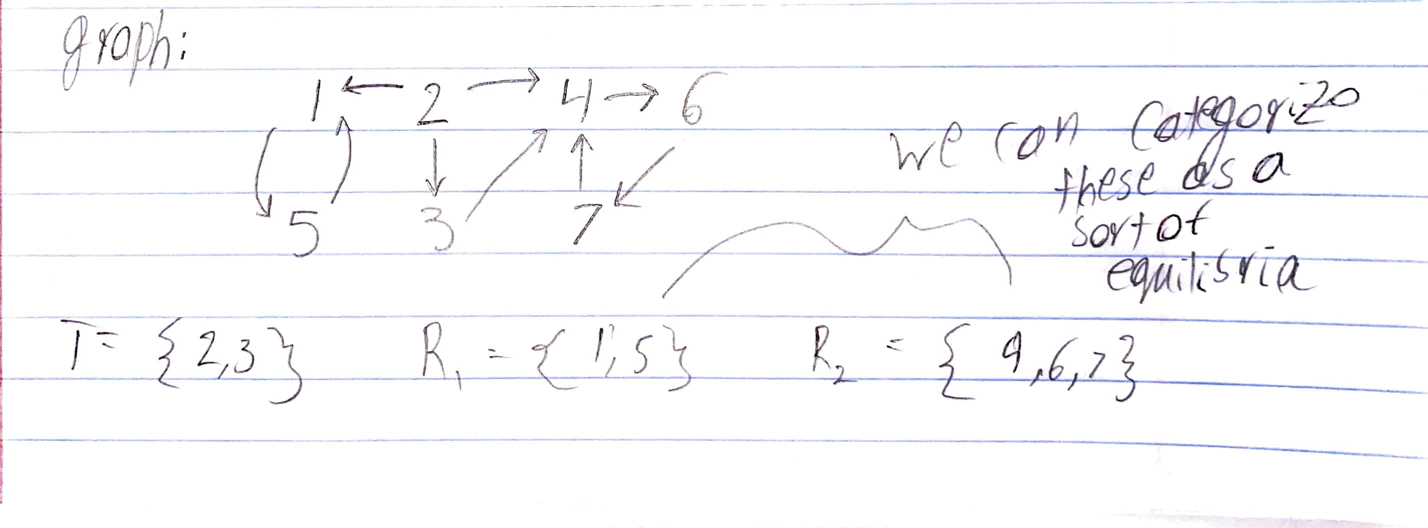
\includegraphics[scale = .5]{example3point2.png}
\end{center}
Note '2' seems to be a pivotal state.
\end{example}


\begin{definition}
  $$
  N(y) := \mid \{ n \geq 1 : X_n = y\} \mid
  $$
  This is the number of visits to $y$ for all $n \geq 1$.
\end{definition}


\begin{lemma}
  \begin{align*}
    \mathbb{E}_x[N(y)] = \frac{\rho_{xy}}{1-\rho_{yy}} = \sum_{n=1}^\infty P_{xy}^n
    \intertext{if this expectation is infinite, then $y$ is recurrent.}
  \end{align*}
\end{lemma}


\begin{corollary}
  $y$ is recurrent $\iff \sum_{n=1}^\infty P_{yy}^n = +\infty$
\end{corollary}

\section{Week 3}
\subsection{Lec 1}

There is another corollary of the previous lemma.

\begin{corollary}
  If $y \in S$ is transient, then

  $$
  \lim_{n \rightarrow \infty} P_{xy}^n = 0
  $$

  $\forall x \in S$.

\end{corollary}

\begin{definition}[\textbf{Stationary distribution}]
  Let there be a vector, $\pi$ such that
$$
  \pi^TP = \pi^T
$$
or in other words, $\pi_j = \sum_{i \in S} \pi_i P_{ij}$.
\end{definition}

We also know that $\lim_{n \rightarrow \infty} P^n,$ if it exists, is a stationary distribution.\footnote{is there a proof for this? Why don't I have it as a separate lemma?} Note $\pi$ is just a left eigenvector with eigenvalue 1. We will explore this connection later in the notes.

\begin{example}
Solving for the stationary distribution is solving for $\pi$ in $\pi^T P = \pi^T.$. Suppose $\pi^T = [\pi_1, \pi_2, \pi_3]$. Then we'll get:

\begin{align*}
  P_{1,1}\pi_1 + P_{2,1} \pi_2 + P_{3,1} \pi_3 = \pi_1 \\
  P_{1,2}\pi_1 + P_{2,2} \pi_2 + P_{3,2} \pi_3 = \pi_2 \\
  P_{1,3}\pi_1 + P_{2,3} \pi_2 + P_{3,3} \pi_3 = \pi_3 \\
\end{align*}

However, because we're solving for a probability vector, all the elements of $\pi$ must add to $1$. This means we introduce the condition $\pi_1 + \pi_2 + \pi_3 = 1$. Solving the four equations yields $\pi$.

\end{example}

\begin{definition}[\textbf{Doubly stochastic matrix}]
  A matrix is called doubly stochastic if its columns also sum to 1. In other words, if $\sum_{i \in S} P_{ij} = 1$ for a fixed $j$.
\end{definition}

\begin{lemma}
  Let $(X_n)_{n=0,1...}$ be a Markov chain on the state space $S = \{1, \dots, N\}$ with doubly stochastic transition matrix $P$. Then the uniform distribution
  \begin{align*}
    \pi_i = \frac{1}{N} && \forall i \in S
  \end{align*}
  is a stationary distribution. \footnote{the proof of this is the solution to problem 1.3.}
\end{lemma}

\begin{definition}[\textbf{Detailed balance condition}]
  Let $P$ be the transition matrix of a Markov chain with state space $S$. We say that a probability vector $\lambda$ satisfies the detailed balance condition if

  \begin{align*}
    \lambda_i P_{ij} = \lambda_jP_{ji} && \forall i,j \in S
  \end{align*}
\end{definition}

\begin{proposition}
  If a probability distribution $\lambda$ satisfies the detailed balance condition, then $\lambda$ is a stationary distribution.
\end{proposition}

\begin{definition}[\textbf{Birth and death chains}]
  There are Markov chains with $S = \{l, l+1, \dots, r-1, r\}$ and transition matrix $P$ such that

  \begin{align*}
    P_{xy} = 0 &&  \text{for  } \mid x -y \mid > 1
    \intertext{and}
    P_{x, x+1} = p_x && \text{for   } x<r \\
    P_{x, x-1} = q_x && \text{for   } x > l \\
    P_{x,x} = 1-p_x-q_x && \text{for   } l \leq x \leq r
  \end{align*}
\end{definition}

\begin{example}
  Here is a 3x3 transition matrix for a birth and death chain.
\begin{align*}
  \begin{bmatrix}
    1 - p_x & p_x & 0 \\
    q_x & 1-p_x - q_x & p_x \\
    0 & q_x & 1 - q_x \\
  \end{bmatrix}
\end{align*}
\end{example}

\begin{proposition}
  Every birth and death Markov chain with $P_{xy} \ne 0 $ for all $x,y \in S$ where $\mid x-y \mid = 1$ has a stationary distribution given by

  \begin{align*}
    \pi_{l + i} = \pi_l * \frac{\prod_{k=1}^i P_{l+k-1, l+k}}{\prod_{k=1}^i P_{l+k, l+k-1}} && \forall i \in \{1, \dots, r - l\}
  \end{align*}
\end{proposition}
\footnote{this is so strange. They use the products in the numerator and denominator but it's just $p_x^i$ and $q_x^i$}

\subsection{Lec 2}
\begin{proposition}
  All Markov chains with a finite state space have at least one stationary distribution. The justification for this is the eigenvalue connection.\footnote{I'd like to investigate this. Perhaps I'll put the proof in.}
\end{proposition}

\begin{proposition}
  An irreducible Markov chain has at most one stationary distribution.
\end{proposition}


The conjunction of these two propositions gives us the following:

\begin{corollary}
  A finite irreducible Markov chain has a unique, positive stationary distribution $\pi$.
\end{corollary}

We're on our way to understanding the limiting behavior of Markov chains. But first, we need the notion of periodicity.

\begin{definition}
  The period of a state $i$ is:
$$
d(i) = \text{gcd}\{n \geq 1: P_{ii}^n > 0\}
$$
A Markov chain (as a whole) is aperiodic if all states have period 1.
\end{definition}

This definition is weird. The period of a state is \textit{not} the length of the shortest cycle that includes it on a transition graph. Nor is it the average number of steps to traverse a cycle on the transition graph. Instead, it's greatest common devisor of the set of lengths of cycles you can make with the state.

A consequence of the greatest common devisor stipulation is that any state that can be revisted in a consecutive number of steps has period 1. For instance, if I can get from $i$ to $i$ in 4 steps and 5 steps, then the period of $i$ is 1.

\begin{lemma}
  Three mini-lemmas.

  \begin{enumerate}
    \item If $P_{ii} >0$, the $d(i) = 1$.
    \item If $x$ and $y$ communicate with each other, then $d(x) = d(y)$. (Lemma 1.17 in Durrett)
  \end{enumerate}
\end{lemma}

\subsection{Lec 3 (limit theorems for Markov chains)}

We're going to refer to these assumptions by the associated abbreviations.

\begin{itemize}
  \item $I$: Markov chain is irreducible
  \item $A$: Markov chain is aperiodic
  \item $R$: All states are recurrent
  \item $D$: There exists a stationary distribution, $\pi$.
\end{itemize}

\begin{theorem}(\textbf{Convergence theorem for Markov chains})
  Say $I, A, D$ are true. then
  \begin{align*}
    \lim_{n \rightarrow \infty} P_x[X_n = y] = \lim_{n \rightarrow \infty} P_{xy}^n = \pi_y
  \end{align*}
  for all $x \in S$.
\end{theorem}

Denote the number of visits to $y$ up to time $n$ as

\begin{align*}
  N_n(y) := \mid \{k \in \{1, \dots, n : X_k = y\} \mid
\end{align*}


\begin{theorem}[\textbf{Asymptotic frequency}]
  Suppose $I$ is true. Then
  $$
  \lim_{n \rightarrow \infty} \frac{N_n(y)}{n} = \frac{1}{E_y[T_y]}
  $$
  for all $y \in S$.
\end{theorem}

\begin{theorem}
  Suppose $I$ and $D$ are true. Then
  $$
\pi_y = \frac{1}{E_y[T_y]}
  $$
  for all $y \in S$.
\end{theorem}

\begin{theorem}[\textbf{Strong law of large numbers for Markov chains}]
  Suppose $I$ and $D$ are true. Let $f: \mathbb{R} \rightarrow \mathbb{R}$ be a function such that $\sum_{x \in S} \mid f(x) \mid \pi_x < \infty$. Then
$$
\lim_{n \rightarrow \infty} \frac{1}{n}\sum_{i=1}^n f(X_i)
 = \sum_{x \in S} f(x)\pi_x
$$
Alternatively, let $Z$ be a discrete random variable with values in $S$ and distribution $\pi$. Then
$$
\lim_{n \rightarrow \infty} \frac{1}{n} \sum_{i =1}^n f(X_i) = E[f(Z)]
$$
\end{theorem}

Compare this with the strong law of large numbers. This is the basis for the Markov Chain Monte Carlo method of estimating the expectation of a random variable.


The following theorem is helpful because it does not assume a finite state space.
\begin{theorem}
  Let $(X_n)_{n=0,1...}$ be an irreducible Markov chain. Then, the following statements are equivalent.
  \begin{enumerate}
    \item There exists a unique stationary distribution
    \item One state is positive recurrent
    \item All states are positive recurrent
  \end{enumerate}
\end{theorem}

All states are automatically positive recurrent for a finite Markov chain.

\section{Week 4}
\subsection{only substantive lecture in the week}

We must review the exponential distribution. We say a random variable $X$ is exponentially distributed by: $X \sim \text{Exp}(\lambda)$ with $\lambda > 0$.

we recall the density function of an exponential.

\begin{align*}
  f_x(x) = \begin{cases}
    \lambda e^{-\lambda x} & x \geq 0 \\
    0 & \text{otherwise}
  \end{cases}
\end{align*}

The cumulative distribution function (CDF) is:

\begin{align*}
  F_x(x) = P(X \leq x) &= \int_{-\infty}^x f_x(y) dy \\
  &= 1-e^{-\lambda x} \\
  \forall x \geq 0
\end{align*}

Additionally, it's helpful to recall the first and second moments.

$$
  \mathbb{E}[X] = \int_{-\infty}^\infty x f_x(x) dx = \frac{1}{\lambda}
$$

and

$$
  \mathbb{E}[X^2] = \int_{-\infty}^\infty x^2 f_x(x) dx = \frac{2}{\lambda^2}
$$

This helps us compute the variance.

$$
  \text{Var}(x) = \mathbb{E}[X^2] - \mathbb{E}[X]^2
  = \frac{2}{\lambda^2} - \frac{1}{\lambda^2} = \frac{1}{\lambda^2}
$$

An important property of exponential distributions is that they are memoryless. Mathematically, we describe this as:
$$
P(X > t + s \mid X > t) = P(X > s)
$$

We can prove this.

\begin{align*}
  P(X > t + s \mid X > t) &= \frac{P(X > t+s, X > t)}{P(X > t)}
  \intertext{We note, as events, $X>t \subset X > t+s$. Hence we rewrite as:}
  &= \frac{P(X > t+s)}{P(X > t)} = \frac{e^{-\lambda (t+s)}}{e^{-\lambda (t)}} \\
  &= e^{-\lambda s} = P(X > s)
\end{align*}

\begin{proposition}
  The exponential distribution is the only continuous memoryless distribution.
\end{proposition}

We now explore the minimum of exponential distributions.

\begin{proposition}
Suppose we have $X \sim \text{Exp}(\lambda)$ and $Y \sim \text{Exp}(\mu)$ and they are independent. Let $M = \text{min}\{X,Y\}$.

Claim (i): $M \sim\text{Exp}(\lambda + \mu)$

Claim (ii): $P(M = X) = \frac{\lambda}{\mu + \lambda} $
\end{proposition}

\begin{proof}
(i)
\begin{align*}
P(M > x) =& P(\text{min}\{X, Y\} > x) = P(X > x, Y > x) = P(X > x)P(Y> x) \\
&= e^{-\lambda x}e^{-\mu x} = e^{-x(\lambda + \mu)}
\end{align*}
which is 1 minus the cdf of Exp$(\lambda + \mu)$

(ii)
\begin{align*}
  P(M = X) &= P(\text{min}\{X, Y\} = X) = P(Y \geq X)
  \intertext{We can use a generalized form of the law of total probability to calculate this.}
  &= \int_0^\infty P(Y \geq X \mid X= x)P(X=x)dx & \\
  &= \int_0^\infty P(Y \geq X \mid X = x)f_x(x) dx \\
  &= \int_0^\infty P(Y \geq x) \lambda e^{-\lambda x} dx \\
  &= \int_0^\infty e^{-\mu x}\lambda e^{-\lambda x} dx = \int_0^\infty  \lambda e^{-x(\mu+\lambda)} \\
  &= \lambda[\frac{-1}{\lambda + \mu}e^{-x(\mu + \lambda)}]_0^\infty = \frac{\lambda}{\lambda + \mu}
\end{align*}
\end{proof}

\section{Week 5}
\subsection{Lec 1}

\begin{proposition}
Suppose $X_1, \dots, X_n$ are $\text{Exp}(\lambda_i)$ and $M = \text{min}\{X_1, \dots X_n\}$.
\begin{enumerate}
  \item for $t > 0$, $P(M > t) = e^{-t(\lambda_1 + , \dots, + \lambda_n)}$. In words, $M$ has an exponential distribution with parameter $\lambda_1 + \dots + \lambda_n$.
  \item for $k = 1, \dots, n$, $P(M = X_k) = \frac{\lambda_k}{\lambda_1 + \dots + \lambda_n}$.
\end{enumerate}

Also, the random variable $M$ and the index of the random variable that is the minimum are independent.
\end{proposition}

\begin{proposition}
  Let $X_1, X_2, \dots X_n$ be independent Exp($\lambda$) random variables. Set $T_n = X_1 + \dots + X_n$. Then $T_n$ has a gamma distribution with parameters $n$ and $\lambda$. The density function is:

$$
f_{T_n}(t) = \lambda e^{-\lambda t}\frac{(\lambda t)^{n-1}}{(n-1)!}
$$

$\forall t> 0$. The mean and variance of $T_n$ are:

\begin{align*}
  \mathbb{E}[T_n] = \frac{n}{\lambda} && \text{Var}(T_n) = \frac{n}{\lambda^2}
\end{align*}
\end{proposition}

We would say $T_n \sim \Gamma(n, \lambda)$.

With this background in place we can finally start to motivate the poisson process. We want to count instances of an event in continuous time. In this sense, we'll say a poisson process is a counting process.

\begin{definition}[\textbf{Counting process}]
  A counting process $(N_t)_{t \geq 0}$ is a collection of non-negative integer-valued random variables such that if $0 \leq s \leq t$ then $N_s \leq N_t$.
\end{definition}

Some notes about counting processes:
\begin{itemize}
  \item Normally, $N_0 = 0$, since we're starting with zero instances of the event.
  \item $N_k$ denotes the number of occurences by time $k$.
  \item for all $ 0 \leq s < t$, $N_t - N_s$ denotes the number of occurences in the time interval $(s, t]$.
\end{itemize}

\begin{definition}[\textbf{Poisson process}]
  A poisson process with $\lambda > 0$ is a continuous time stochastic process with the following properties:
  \begin{enumerate}
    \item $N_0 = 0$
    \item (independent increments)$\forall n \in \mathbb{N}$, $0 \leq t_1 < t_2 < \dots < t_n$, the random variables $N_{t_2} - N_{t_1}, N_{t_3} - N_{t_2}, \dots, N_{t_n} - N_{t_{n-1}}$ are independent.
    \item (stationary increments) for all $0 \leq s < t$ the random variable $N_t - N_s$ is a poisson distribution with parameter $\lambda(t-s)$.
    \item (redundant property) the function $t \mapsto N_t$ is a right-continuous step function with jump size 1.
    \end{enumerate}
\end{definition}

property 4 just means the poisson process jumps by at most 1 (check this).

Several consequences flow from these properties.

\begin{itemize}
  \item $N_t = N_t - 0 = N_t - N_0 \sim \text{Pois}(\lambda t)$ $\forall t > 0$.
  \item $\mathbb{E}[N_t] = \lambda t$ ($\lambda$ is called the arrival rate)
\end{itemize}

We must note that $N_t$ is not independent of $N_s$. Only the difference is independent from other, non-overlapping differences.

\subsection{Lec 2}

Recall $N_i$'s are poisson distributed with parameter $\lambda_i$ where $i$ is the time interval. We can see this by seeing:
\begin{align*}
  N_t = N_t - N_s + N_s - N_0 \sim \text{Pois}(\lambda(t-s) + \lambda s) = \text{Pois}(\lambda t)
\end{align*}

\begin{example}
  Students come to the library at the rate 30 per hour starting at 6am. What is the probability more than 65 arrive between 9am and 11am?

  \underline{solution}
  Let $N_t = $ the number of students who have arrived at the library by time $t$. $(N_t)_{t \geq 0}$ is a poisson process with $\lambda > 0$. Stipulate time is measured in hours. Then $\lambda = 30$ and $t_0 = $ 6am, $t_3 = $ 9am and $t_5 = $ 11am.

  In these terms, our problem becomes calculating $P(N_5 - N_3 > 65)$. By stationary increments, we know $N_5 - N_3$ is poisson distributed with $\lambda = 2(30)$. Hence, we compute $P(\text{Pois}(60) > 65)$.

  It's easy enough to plug this into a calculator, or wolfram, or whatever, but it's worth manipulating it a little to see what different forms this expression can take. We know $N_2 \sim \text{Pois}(60)$, so we can replace it.
  \begin{align*}
    P(\text{Pois}(60) > 65) = P(N_2 > 65) &= 1-P(N_2 \leq 65) \\
    &= 1-\sum_{k \leq 65}P(N_2 = k)
    \intertext{we know the PMF of $N_2$ since it is Pois$(60)$}
    &= 1 - \sum_{k \leq 65}e^{-60}\frac{60^k}{k!}
  \end{align*}
  In the end, the probability comes out to be $\approx .235$.
\end{example}

\begin{example}
  Visitors to a website start arriving at 10am every morning and come at a rate of 10 per hour according to a Poisson process.

  \begin{enumerate}
    \item What's the probability you will get exactly 18 visitors by noon and exactly 70 by 5pm?
    \item Suppose you received exactly 18 visitors by noon. Find the probability you will get exactly 70 visitors by 5pm.
  \end{enumerate}

\underline{Solution}
The first question is asking for the probability of two events. We can express this as: $P(N_2 - N_0 = 18, N_7 - N_2 = 52)$. We set $N_7 - N_2 = 52$ because in order to get 70 visitors by 5, we need to get 18 from 10 to noon, and 52 from noon to 5. By independent increments, we split up the probability.

\begin{align*}
  &= P(N_2 - N_0 = 18)P(N_7 - N_2 = 52) = P(\text{Pois}(20) = 18)P(\text{Pois}(50) = 52) \\
  \intertext{The Poisson distributions replace the differences due to the stationary increments property}
  & = e^{-20}\frac{20^{18}}{18!} * e^{50}\frac{50^{52}}{52} \\
  &\approx .084 * .053
\end{align*}

The second question asks for a conditional probability. We want to find $P(N_7  = 70 \mid N_2 = 18)$. Approach this by using the definition of conditional probability.

\begin{align*}
  &= \frac{P(N_7 = 70, N_2 = 18)}{P(N_2 = 18)} \\
  &= P(N_7 - N_2 = 52) \\
  &= P(N_5 = 52) = P( \text{Pois}(50) = 52) \\
  &\approx .053
\end{align*}

\end{example}

\subsection{Bonus Section (indicator functions and expectation)}

Indicator functions help us convert between events and random variables. From an event, $A$, we want to get a random variable $1_A$ that takes the value 1 if $A$ obtains and 0 otherwise.

\begin{align*}
  1_A = \begin{cases}
    1 & A \\
    0 & \neg A
\end{cases}
\end{align*}

We note $\mathbb{E}[1_A] = P(A)$.

To go the other way around, from random variables to events, we notice for a random variable $X$,

$$
X = \sum_x x*1[X = x]
$$

Think about what a random variable is. It takes on certain values with a given probability. Hence, we can split up all the possible values and pick the one that the random variable actually takes (this is accomplished by $1[X=x]$). We multiply all the other values by zero, add it to the value actually obtained, and we get the same result as a standard random variable.

\begin{proposition} This allows us to put a conditional expectation into something more manageable.
  \begin{align*}
    \mathbb{E}[X \mid B] &= \mathbb{E}[\sum_x x 1[X=x] \mid B]
    \intertext{by linearity of expectation we can pull out the sum}
    &= \sum_x x \mathbb{E}[1[X = x] \mid B] \\
    &= \sum_x x \frac{\mathbb{E}[1[X = x \cap B]]}{P(B)} \\
    & = \frac{1}{P(B)} \mathbb{E}[\sum_x x 1[X = x]1[B]]\\
    &= \frac{\mathbb{E}[X 1[B]]}{P(B)}
  \end{align*}
\end{proposition}

\begin{example}
  Let $X$ and $Y$ be two independent exponentially distributed random variables with parameters $\lambda > 0$ and $\mu > 0$, respectively. Show

  $$
  \mathbb{E}[\text{min}\{X, Y\} \mid X<Y] = \frac{1}{\lambda + \mu}
  $$

  \underline{Solution}
  From the prior proposition, we know

  $$
  \mathbb{E}[\text{min}\{X,Y\} \mid X<Y] = \frac{\mathbb{E}[\text{min}\{X,Y\}] 1[X<Y]}{P(X < Y)}
  $$

  We proceed by looking at the numerator.

  \begin{align*}
    \mathbb{E}[\text{min}\{X,Y\}] 1[X<Y]P(X < Y)] &= \mathbb{E}[X 1[X < Y]] \\
    &= \int \int_{\mathbb{R}} x 1[X < Y] \mu \lambda e^{-x\lambda}e^{-y \mu} dy dx \\
    &= \int_0^\infty \int_0^\infty x 1[X <Y] \mu \lambda e^{-x\lambda}e^{-y \mu} dy dx \\
    &= \int_0^\infty x \lambda e^{-x\lambda} dx \int_x^\infty \mu e^{-y \mu} dy \\
    &= \int_0^\infty x \lambda e^{-x \lambda} * e^{-x\mu}dx \\
    &=  \int_0^\infty x \lambda e^{-x(\lambda + \mu)} dx \\
    &= \frac{\lambda}{\lambda + \mu} (\lambda + \mu e^{-x(\lambda + \mu)} dx \\
    &= P(X < Y) \mathbb{E}[Z]
  \end{align*}

  where $Z \sim \text{Exp}(\mu + \lambda)$. Now we can plug it into the original equation.

  \begin{align*}
    \mathbb{E}[\text{min}\{X,Y\} \mid X<Y] = \frac{P(X < Y) \mathbb{E}[Z]}{P(X<Y)} = \mathbb{E}[Z] = \frac{1}{\lambda + \mu}
  \end{align*}
\end{example}

\textbf{Add the correlation problem}

\subsection{Lecture 3}

There is a different way to look at Poisson processes. We "decompose" them so to speak into the arrival times of events, and the times in between arrivals.

\begin{proposition}
  Let $\tau_1, \tau_n \dots$ be a sequence of iid exponential random variables with parameter $\lambda > 0$. Also, let $T_n = \tau_1 + \dots + \tau_n$ and $T_0 = 0$ for $n \geq 1$. For $t \geq 0$ let

  $$
N_t = \text{max}\{n \geq 0: T_n \leq t\} = \sum_{k=1}^n 1_{(0,t]}(T_k)
  $$

  Then $N_t$ is a poisson process with parameter $\lambda > 0$.
\end{proposition}

$T_i$ is the arrival time of the $i$th event in the poisson process. For instance, if the 8th patron enters a store according to a poisson process at time 40, then $T_8 = 40$. $\tau_i$ represents the time between $T_i$ and $T_{i-1}$. If $T_7 = 30$ then $\tau_8 = 10$.

This leads us to the next proposition.

\begin{proposition}
  Let $N_t$ be a poisson process with parameter $\lambda > 0$. For some $t> 0$ let $N_t = n$ and have $T_1 \dots T_n$ be the corresponding arrival times.

  Also, let $U_1 \dots U_n$ be iid uniform random variables on $[0,t]$. Then:

  $$
(T_1, \dots, T_n \mid N_t = n) = (U_{(1)}, \dots , U_{(n)})
  $$
  In distribution, where $U_{(i)}$ is the $i$th order statistic of the iid uniform random variables.\footnote{The statement of this proposition is altered a bit from Voss' class materials. He expresses the thought in words several times before givng a more concise mathematical formulation. This proposition is 2.10 in the slides (and probably in the Durrett book)}
\end{proposition}

The proposition says something powerful. If we know the value of $N_t$ at some time $t$, then we can say something useful about the joint distribution of arrival times. In particular, we know the joint distribution is identical to the joint distribution of $n$ uniform random distributions on the interval $[0,t]$. We know that that is:

$$
f(u_1, u_2, \dots, u_n) = \begin{cases}
  \frac{n!}{t^n} & \text{ if } 0 \leq t_1 \leq t_2  \leq  \dots \leq t_n < t \\
  0 & \text{otherwise}
\end{cases}
$$

Here are some examples of general problem-solving with poisson processes. Note they don't necessarily make us of the propositions we just covered.

\begin{example}
  The times when goals are scored in hockey can be modeled as a Poisson process. Assume such a process where the average time between goals is 15 minutes.

  \begin{enumerate}
    \item In a 60-minute game, find the probability that a fourth goal occurs in the last 5 minutes of the game
    \item Assume at least three goals are scored in a game. What is the mean time of the third goal
  \end{enumerate}

  \underline{Solution} 1)

  We're seeking $P(55 <T_4 < 60)$. Recall $T_4$ is gamma distributed.\footnote{This is because $T_n = \tau_1 + \tau_2 \dots$ where $\tau$ is an exponential random variable. The sum of n iid exponential random variables is $\Gamma (n, \lambda)$} This means we can evaluate the expression directly as:
  $$
  \int_{55}^{60} (1/15)e^{-t/15} \frac{(t/15)^3}{3!} dt \approx .068
  $$

  2) We're looking for: $\mathbb{E}[T_3 \mid T_3 < 60]$. We recall a formula for conditional expectation covered in section 6.3. Hence,

  \begin{align*}
    &\mathbb{E}[T_3 \mid T_3 < 60] = \frac{1}{P(T_3 < 60)} \mathbb{E}[T_3 1_{T_3 < 60}]
    \intertext{We know $P(T_3 < 60)$ is evaluable because its gamma distributed. Looking closely at the expectation, we realize for all $T_3 > 60$ the indicator function will be 0. Hence, we can 'cut off' the expectation at 60.}
    &= (\int_0^{60} \frac{1}{15}e^{-t/15} \frac{(t/15)^2}{2!} dt )^{-1} *  \int_0^{60}t \frac{1}{15}e^{-t/15} \frac{(t/15)^2}{2!} dt
    \intertext{Going through the calculation, we see this comes out as:}
    & \approx 33.46
  \end{align*}
\end{example}

\begin{example}
  Starting at $t=0$ patrons arrive at a restaurant according to a possion process with a rate of 20 customers per hour.

  If 60 people arrive at the restaurant by time $t=3$, find the probability that the 60th customer arrives in the interval $[2.9, 3]$.

  \underline{Solution} Formally, we're after $P(T_{60} \in [2.9,3] \mid N_3 = 60)$. In words, this is the probability the 60th customer arrives between $t= 2.9$ and $t= 3$.

  We use proposition 6.5 to say:

  $$
  (T_{60} \in [2.9,3]) = (U_{(60)} \in [2.9, 3])
  $$

  in distribution. Hence,

  \begin{align*}
    P(T_{60} \in [2.9,3] \mid N_3 = 60) &= P(U_{(60)} \in [2.9,3]) \\
    &= {P(U_{(60)} > 2.9)}
    \intertext{The last step is valid since 3 is the end of the interval the $U$'s are distributed on.}
    &= 1- P(U_{(60)} < 2.9)
    \intertext{Notice $U_{(60)}$ is an order statistc. This means that if $U_{(60)} < 2.9$, then all of the 60 iid $U$'s must also be below 2.9.}
    &= 1- P(U_1 < 2.9, U_2 < 2.9, \dots, U_60 < 2.9) \\
    &= 1- (\int_0^{2.9} \frac{1}{3} dt)^{60}\\
    &= 1- \frac{2.9}{3}^{60}\\
    &\approx .869
  \end{align*}
\end{example}

\section{Week 6}
The first lecture of week 6 was a continuation of the lecture 3 week 5. We did the same problems. The second lecture didn't happen because it was Veteran's day. I skip to Jacob's section.

\subsection{Jacob's section}

\begin{example}
  Consider a series of payments of \$ 1000 at the random arrival times of a Poisson process with parameter $\lambda > 0$. Recall that if the continuously compounded interest rate is $r > 0$ the nthe present value at time 0 of a payment of \$ 1000 at some future point in time $t > 0$ is given by \$ 1000 $* e^{-rt}$.

  Demonstrate the expected present value at time 0 of the random series of payments until $T > 0$ is $1000 \lambda (1-e^{-rT}) /r $.

  \underline{Solution} Let $X$ be the random variable representing the present value of the future payments. For some $T$, there will be $N_T$ payments of 1000 on the interval $[0,T]$. The value of $X$ is just the sum of these payments discounted to the present. What's more, a payment arriving at $T_k$ will be worth $1000 e^{-rT_k}$ at time 0. Hence,

  $$
  X = \sum_{k=1}^{N_T} 1000 e^{rT_k}
  $$

  Now, we use the law of total expectation to get the expected value of $X$. Recall the law is:\footnote{There's a condition $Y$ has to fulfill. Check this and include it. }

  $$
\mathbb{E}[X] = \sum_{k=0}^{\infty} \mathbb{E}[ X \mid Y = k] P(Y = k)
  $$

  Hence,
  \begin{align*}
    \mathbb{E}[X] &= \sum_{n=0}^{\infty} \mathbb{E}[ \sum_{k=1}^{N_T} 1000 e^{rT_k} \mid Y = n] P(Y = n)
    \intertext{The law of total expectation allows us to replace $Y$ with any discrete random variable that takes positive natural values. Condition on $N_T = n$ since we're holding a time fixed and caluclating expected value from that.}
    & = \sum_{n=0}^{\infty} \mathbb{E}[ \sum_{k=1}^{n} 1000 e^{rT_k} \mid N_T = n] P(N_T = n)\\
    \intertext{We know that $N_T$ is a Poisson so we can replace.}
    & = \sum_{n=0}^{\infty} \mathbb{E}[ \sum_{k=1}^{n} 1000 e^{rT_k} \mid N_T = n] \frac{(\lambda T )^n e^{-\lambda T}}{n!}
    \intertext{Recall Proposition 6.5. We're going to use it to replace all the $T_k$'s with uniform normals. Rigorously, we say:}
    &\text{let } \{A_1 , A_2 \dots A_n\} \sim \text{Uniform}(0,T). \\
    &\text{Put them in order, like so: } A_{j_1} \leq A_{j_2} \leq \dots \leq A_{j_n}
    \intertext{by proposition 6.5, we know $\{A_{j_k} \}_k = \{T_k \mid N_T = n \}$ in distribution. Now, we can make the swap.}
    & \mathbb{E}[ \sum_{k=1}^{n} 1000 e^{rT_k} \mid N_T = n] = \mathbb{E}[ \sum_{k=1}^n 1000 e^{-r A_{jk}}] = \mathbb{E}[ \sum_{k=1}^n 1000 e^{-r A_{j}}] \text{(by iid)}
    \intertext{notice there is no dependence on $k$. We can pull out the relevant terms.}
    & = n1000 \mathbb{E}[e^{-rA_{j}}] \\
    &= 1000n \int_{0}^{\infty} e^{-ra} \text{PDF}(A_j = a) da
    \intertext{but remember, $A_j$ is a normal on the interval $[0, T]$}
    & = 1000n \int_{0}^{T} e^{-ra} \frac{1}{T} da \\
    & = 1000n \frac{1-e^{-rT}}{rT}
    \intertext{Now we make the substitution}
    & = \sum_{n=0}^{\infty} 1000n \frac{1-e^{-rT}}{rT} \frac{(\lambda T)^n e^{-\lambda}}{n!} = 1000  \frac{1-e^{-rT}}{rT} \sum_{n=0}^{\infty}  n \frac{(\lambda T )^n e^{-\lambda T }}{n!}
    \intertext{notice the sum is just the expectation of a Poisson with mean $\lambda T$.}
    & = 1000  \frac{1-e^{-rT}}{rT} \lambda T = 1000 \lambda \frac{1-e^{-rT}}{r}
  \end{align*}

  as desired.

  \end{example}

  \begin{example}
    Babies are born at a maternity ward according to a Poisson process with $\lambda >0 $.

    The the babies' sexes are indpendent of each other (having a boy does not make a girl more likely). According to the UN, the global sex ration for boys to girls is $p = .519$.

    How can the number of male and female births in the maternity ward be described?


    \underline{Solution} This is a strangely phrased question. Essentially, it's asking us to play around the with equation for a Poisson process while 'keeping track' of a single sex and to see what happens.

    Let $N_t$ be the the total number of babies born by time $t$ and let $M_t$ and $F_t$ be the number of babies born by $t$ with male and female sexes, respectively.

    Let's compute the joint distribution of $P(M_t = m, N_t = m+f)$.

    \begin{align*}
      &P(M_t = m, N_t = m+f) = P(M_t = m \mid N_t = m+f)P(N_t = m+f)
      \intertext{The last term is Poisson distributed so we hold off for now}
      \intertext{We treat births like Bernoulli trials with $ p = .519$. Hence, the probability of getting $m$ successes in $m+f$ Bernoulli trials is}
      & {m + f \choose m} P(\text{male})^m P(\text{female})^f
      \intertext{replace $P(M_t = m \mid N_t = m+f)$ with the previous expression.}
      & ={m + f \choose m} P(\text{male})^m P(\text{female})^f P(N_t = m+f) \\
      & = {m + f \choose m} P(\text{male})^m P(\text{female})^f \frac{(\lambda t)^{m+f} e^{-\lambda t}}{(m+f)!} \\
      &= \frac{(m+f)!}{m!f!} (\lambda t)^m (\lambda t)^f \frac{1}{(m+f)!}
      \intertext{notice we can multiply the exponent of the exponential by 1, or $P(\text{male}) + P(\text{female})$.} \\
      &= \frac{(t \lambda P(\text{male}))^m  e^{-\lambda t P(\text{male})}}{m!}
      \frac{(t \lambda P(\text{female}))^f e^{-\lambda t P(\text{female})}}{f!} \\
      & = \text{Pois}(P(\text{male})\lambda ) * \text{Pois}(P(\text{female}) \lambda)
      \intertext{which is two Poisson distributions. This suggests that if we categorize different types of arrivals in a Poisson process, they are also Poisson distributed.}
    \end{align*}
  \end{example}


  \subsection{Lec 3}

  We will talk about thinning and superpositioning of Poisson processes

  \begin{proposition}
    Let $(N_t)_{t \geq 0}$ be a Poisson process with parameter $\lambda > 0$. Assume that each arrival, indpendent of other arrivals, is marked as a type $k$ event with probability $p_k \in (0,1)$, for $k = 1, 2, \dots, n$, where $p_1 + p_2 + \dots + p_n =1$.

    Let $(N^{(k)})_t$ be the number of type $k$ events in $[0,t]$. Then, $(N^{(k)}_t)_{t \geq 0}$ is a Poisson process with parameter $\lambda p_k > 0$.

    Additionally, the processes,

    $$
    (N^{(1)}_t)_{t \geq 0}, \dots,  (N^{(n)}_t)_{t \geq 0}
    $$

    are independent. Each is called a thinned Poisson process. We also notice $N^{(1)}_t + N^{(2)}_t + \dots + N^{(n)}_t  =  N_t$.
  \end{proposition}

  We can see a special case of this in birth example in the previous section.

  \begin{proposition}
    Assume that

    $$
(N^{(1)}_t)_{t \geq 0}, \dots,  (N^{(n)}_t)_{t \geq 0}
    $$

    Are $n$ indpendent Poisson processes with respective parameters $\lambda_1, \dots, \lambda_n > 0$. Let

    $$
    N_t = N^{(1)}_t + N^{(2)}_t + \dots + N^{(n)}_t
    $$

    Is a Poisson process with parameter $\lambda = \lambda_1 + \lambda_2 + \dots + \lambda_n$.

    We call this the superpositioning process.
  \end{proposition}

  There are several ways to simulate a Poisson distribution.

  \underline{Method 1}
  This method relies on the idea a Poisson process is composed of stationary increments.
  \begin{enumerate}
    \item Split $[0,T]$ into $n$ small subintervals of length $\Delta t = T/n$. $\Delta t$ must be sufficiently small such that the probability of getting 2 occurrences from a Poisson random variable on it is very low.
    \item create $n$ iid Poisson random variables $\Delta N_1, \Delta N_2, \dots, \Delta N_n$ with parameter $\lambda \Delta t$
    \item Let $N_0 = 0$. For each $i = 0, \dots, n-1$ let $N_{(i +1)\Delta t} = N_{i \Delta t} +\Delta  N_{i +1}$
    \item For all $i = 0, \dots, n-1$ and each $t \in [i \Delta t, (i+1) \Delta t)$, set $N_t = N_{i \Delta t}$.
  \end{enumerate}

  \underline{Method 2}
  This method relies on the idea the interarrival times for a Poisson process are exponentially distributed.

  \begin{enumerate}
    \item Let $T_0 = 0$.
    \item Generate iid exponential random variables $\tau_1, \tau_2, \dots,$ with parameter $\lambda$.
    \item Let $T_n = \tau_1 + \dots + \tau_n$ for $n = 1, 2, \dots$.
    \item For each $k = 0, 1, \dots$ let $N_t = k$ for $T_k \leq t < \text{min}\{T_{k+1}, T\}$.
  \end{enumerate}

  \underline{Method 3}
  This one relies on the fact the arrival times are normally distributed on the interval.

  \begin{enumerate}
    \item Simulate the total number of arrivals on $[0,T]$ from a Poisson distribution with parameters $\lambda T$.
    \item Generate $N_t = n$ iid random variables $U_1, \dots, U_n$ uniformly distributed on $[0,T]$.
    \item Sort the variables in increasing order (make order statistics) in order to get the arrival times.
    \item For each $k = 0, 1 \dots, n-1$ set $N_t = k$ for $T_k \leq t < T_{k+1}$ and set $N_t = n$ for $T_n \leq t < T$.
  \end{enumerate}

We're going to introduce a more realistic Poisson process. In this model, the $
\lambda$ changes as time varies. We might call this a nonhomogeneous Poisson process.

\begin{definition}[Nonhomogeneous Poisson Process]

  A counting process is a nonhomogeneous Poisson process with intensity function $\lambda(t)$ if
  \begin{enumerate}
    \item $N_0 = 0$
    \item (independent increments) For all $n \in \mathbb{N}, 0 \leq t_1 < t_2 < \dots < t_{n}$ the random variables $N_{t_i} - N_{t_{i-1}}$ are independent.
    \item For all $0 \leq s < t$ the random variable $N_t - N_s$ is Poisson distributed with parameter $\int_{s}^t \lambda(u) du $
  \end{enumerate}

\end{definition}

We no longer have stationary distributions anymore. Furthermore, if $\lambda$ is a constant we have a regular Poisson process.

\begin{definition}[Compound Poisson Process]
  Let $(N_t)_{t \geq 0}$ be a Poisson process with $\lambda > 0$. Furthermore, let $Y_1, \dots$ be a sequence of iid random variables with density function $f_y$, also independent of $(N_t)_{t \geq 0}$. Then,

  $$
C_t = \sum_{i =1}^{N_t} Y_i
  $$
  for $t \geq 0$ is a compound Poisson process with jump-distribution $f_y$ and jump intensity $\lambda$.

\end{definition}

\section{Week 7}
\subsection{Lecture 1}

We will be finishing up Poisson processes and then moving onto renewal processes.

Recall what we've said about compound Poisson processes. We introduce and additional fact.

\underline{Fact}
If we have a compound Poisson process, $C_t$, then the following are true.
\begin{enumerate}
  \item $C_0 = 0$
  \item $C_t$ has independent increments in the same way a regular Poisson process does.
  \item The increments are stationary (though they are no long Poisson distributed)
\end{enumerate}

Now, we have an example that makes use of these properties.

\begin{example}
  Let $(C_t)_{t \geq 0}$ be a compound Poisson process.
  Show:
  \begin{enumerate}
    \item $\mathbb{E}[C_t] = \lambda t \mathbb{E}[Y_1]$
    \item compute $\text{Var}(C_t)$.
  \end{enumerate}

\underline{Solution}
First, in order to do this problem we must assume $\mathbb{E}[Y_1] < \infty , \mathbb{E}[Y_1^2] < \infty, \mathbb{E}[N] < \infty , \mathbb{E}[N^2] < \infty$.

1) We recall and apply the law of total expectation.

\begin{align*}
  \mathbb{E}[C_t] &= \mathbb{E}[\sum_{i=1}^{N_t} Y_i] = \sum_{k = 0}^\infty \mathbb{E}[\sum_{i=1}^{N_t} Y_i \mid N_t = n]P(N_t = n) \\
  \intertext{We look at the conditional expectation and realize it fixes some $n$ where the internal sum ends. Thus, we can replace a random sum with a deterministic sum.}
  &= \sum_{k = 0}^\infty \mathbb{E}[\sum_{i=1}^{n} Y_i]P(N_t = n)
  \intertext{We can bring the sum outside of the second expectation since the $Y_i$'s are independent of $n$. The $Y_i$'s are also iid, which allows us to replace them all with $Y_1$.}
  &= \sum_{k = 0}^\infty n \mathbb{E}[Y_1] P(N_t = n) \\
  &=  \mathbb{E}[Y_1] \sum_{k = 0}^\infty n P(N_t = n) \\
  &= \mathbb{E}[Y_1] \mathbb{E}[N] = \mathbb{E}[Y_1] \lambda t
\end{align*}

As desired.

2) Computing the variance is a bit tougher. We recall that $\text{Var}(C_t) = \mathbb{E}[C_t^2] - \mathbb{E}[C_t]^2$. We already know $\mathbb{E}[C_t]^2$, so it remains to compute $\mathbb{E}[C_t^2]$. We use the law of total expectation again.

\begin{align*}
  \mathbb{E}[C_t^2] &= \sum_{k=0}^\infty \mathbb{E}[C_t^2 \mid N_t = k]P(N_t = k) \\
  &= \sum_{k=0}^\infty \mathbb{E}[(\sum_{i = 1}^{N_t} Y_i)^2 \mid N_t = k]P(N_t = k)
  \intertext{from here, we use the law of conditional variance to calculate the conditional expectation. Recall for some random variable $S$,}
  & \text{Var}(S \mid N_t = n) = \mathbb{E}[S^2 \mid N_t = n] - \mathbb{E}[S \mid N_t = n]^2
  \intertext{Now, we solve for the conditional expectation of the second moment substitute.}
  &\mathbb{E}[C_t^2 \mid N_t = k] = \text{Var}(C_t \mid N_t = k) + \mathbb{E}[C_t \mid N_t = k]^2 \\
  &= \text{Var}(\sum_{i = 1}^{N_t} Y_i \mid N_t = k) + \mathbb{E}[\sum_{i = 1}^{N_t} Y_i \mid N_t = k]^2 \\
  & = \text{Var}(\sum_{i = 1}^{k}Y_i) + \mathbb{E}[\sum_{i = 1}^{k} Y_i]^2 \\
  &= k \text{Var}(Y_1) + k^2 \mathbb{E}[Y_i]^2
  \intertext{we plug in now.}
  \mathbb{E}[C_t^2] &= \sum_{k=0}^\infty (k \text{Var}(Y_1) + k^2 \mathbb{E}[Y_i]^2) P(N_t = k) \\
  &= \sum_{k=0}^\infty kP(N_t = k)\text{Var}(Y_1) + k^2P(N_t = k)\mathbb{E}[Y_1]^2 \\
  \intertext{Bring the sums in}
  &=\text{Var}(Y_1) \sum_{k=0}^\infty kP(N_t = k) + \mathbb{E}[Y_1]^2 \sum_{k=0}^\infty k^2 P(N_t = k) \\
  &=\text{Var}(Y_1)\mathbb{E}[N_t] + \mathbb{E}[Y_1]^2 \mathbb{E}[N_t^2]
  \intertext{We now subtract $\mathbb{E}[C_t]^2$ to get the variance}
  \text{Var}(C_t) &= \text{Var}(Y_1)\mathbb{E}[N_t] + \mathbb{E}[Y_1]^2 \mathbb{E}[N_t^2] - \mathbb{E}[Y_1]^2 \mathbb{E}[N_t]^2 \\
  &= \text{Var}(Y_1) \mathbb{E}[N_t] + \mathbb{E}[Y_1]^2(\mathbb{E}[N_t^2] - \mathbb{E}[N_t]^2) \\
  &= \text{Var}(Y_1)\mathbb{E}[N_t] + \mathbb{E}[Y_1]^2\text{Var}(N_t) \\
  &= \lambda t \text{Var}(Y_1) + \mathbb{E}[Y_1]^2 \lambda t \\
  &= \lambda t (\text{Var}(Y_1) + \mathbb{E}[Y_1]^2) \\
  &= \lambda t \mathbb{E}[Y_1^2]
\end{align*}

Which finishes the problem.

\end{example}

Here is a proposition that allows us to pass from compound Poisson processes to regular ones. It is very similar to our proposition that details 'thinning' regular Poisson processes.

\begin{proposition}
  Let $(C_t)_{t \geq 0}$ be a compound Poisson process with jump intensity $\lambda$ and jump distribution $f_Y$. Also, let $A_1, A_2, \dots A_n$ be pairwise disjoint subsets of $\mathbb{R}$ and let

  $$
  N_t^{(k)} = \sum_{i=1}^{N_t} 1_{\{Y_i \in A_k\}}
  $$

   for all $k=1, \dots, n$ where $t \geq 0$. Then,

  $$
  (N_t^{(1)})_{t \geq 0},   (N_t^{(2)})_{t \geq 0} \dots   (N_t^{(n)})_{t \geq 0}
  $$
  are independent Poisson processes with rate $\lambda P(Y_1 \in A_k)$.
\end{proposition}

\subsection{Lec 2}

We have the basic components of a Poisson process down. We know arrivals over an interval follow a Poisson distribution with paratmeter $\lambda t $ and the interarrival times are exponentially distributed (which implies the arrival times ares gamma distributed). What happens if we relax one of these assumptions? For instance, we might want to model something where it doesn't make sense to say the interarrival times are exponentially distributed. It might be the case the longer you wait for an arrival, the more likely it is going to come in a relatively short time span.

In this case, we are dealing with a renewal process.

\begin{definition}[Renewal process]
  Let $L_1, L_2, \dots$ be a sequence of positive iid random variables. We call $L_i$ the $i$-th holding time and $(L_i)_{i = 1, 2 \dots} $ the renewal sequence.

  Let $T_0 = 0$ and define $T_n = \sum_{i=1}^n L_i$ for all $n \geq 1$. Each $T_n$ is referred to as the $n$-th jump time, and $[T_n, T_{n+1}]$ as the renewal interval.

  For $t \geq 0$ let

  $$
  N_t = \text{max}\{n \geq 0: T_n \leq t\} = \sum_{k=1}^\infty 1_{(0,t]} T_k
  $$

  Then $N_t$ represents the number of jumps that have occurred by time $t > 0$ and the continuous-time stochastic process $(N_t)_{t \geq 0}$ is called a renewal process.

\end{definition}

Notice the $L_i$'s are comparable to a sequence of exponential random variables we might have had in a regular Poisson process. The difference here is that the $L_i$'s can be distributed in any fashion, now. The fact the renewal sequence is not exponentially distributed means the jump times, or arrival times ($T_i$) are no longer gamma distributed.

\begin{example}
  This is just meant to give you an idea of what renewal processes can model.

  We might use such a process to model the breakdowns of parts in a machine.
  \begin{itemize}
    \item Let $L_1, L_2 \dots $ be the lifetimes of the parameters
    \item $T_n$ is the breakdown of the $n$-th part.
    \item $N_t$ is the number of parts replaced in a machine by time $t$.
  \end{itemize}
\end{example}

Since renewal processes are more general, it's more difficult to know things about them.\footnote{or so i've been told.} Consequently, we're left with asymptotic results.

\begin{theorem}
  Let $(N_t)_{t \geq 0}$ be a renewal process. Then

  $$
\lim_{t \rightarrow + \infty} \frac{N_t}{t} = \frac{1}{\mathbb{E}[L_1]}
  $$
\end{theorem}

\begin{proof}
  First, recall the strong law of large numbers. For $L_1, L_2, \dots$,
  $$
\frac{1}{n} \sum_{i = 1}^\infty L_i \rightarrow \mathbb{E}[L_1]
  $$
  As $n \rightarrow \infty$. We also note that $N_t \rightarrow \infty$ as $t \rightarrow \infty$.

  What follows is the crucial move of the proof. Observe that

\begin{align*}
  T_{N_t} &\leq t < T_{N_t + 1}
  \intertext{In words, the arrival time of the $N_t$-th arrival is going to be less than or equal to the time $t$. This is intuitive, since the last arrival happening at a time before $t$ cannot occur at a time after $t$. Now, we realize that the arrival time of $N_t + 1$ must happen after $t$. If it happened at $t$ or prior, it must count towards $N_t$. Now we manipulate the inequality.}
  & \iff \frac{T_{N_t}}{N_t} \leq \frac{t}{N_t} < \frac{T_{N_t + 1} (N_t + 1)}{N_t * (N_t + 1)}
  \intertext{take the limit as $t \rightarrow \infty$. We use the fact $N_t \rightarrow \infty$ as $t \rightarrow \infty$ to invoke the law of large numbers.}
  &\iff \mathbb{E}[L_1] \leq \frac{t}{N_t} < \lim_{t \rightarrow \infty} \frac{T_{N_t} + 1}{N_t + 1} * \frac{N_t  +1}{N_t } \\
  &\iff \mathbb{E}[L_1] \leq \frac{t}{N_t} < \mathbb{E}[L_1]*1 \\
  &\iff \lim_{t \rightarrow \infty} \frac{t}{N_t} = \mathbb{E}[L_1]
  \intertext{Take the reciprocal and we get}
  & \lim_{t \rightarrow \infty} \frac{N_t}{t} = \frac{1}{\mathbb{E}[L_1]}
  \intertext{As desired}
\end{align*}
\end{proof}

Here is a quick application of the result, applied to our familiar Poisson process.

\begin{example}
  Let $N_t$ be a Poisson process with parameter $\lambda > 0$. Then

  $$
\lim_{t \to \infty } \frac{N_t}{t} = \frac{1}{\mathbb{E}[L_1]} = \frac{1}{1/\lambda} = \lambda
  $$
\end{example}

Now, we want to talk about coninuous time Markov chains. What's the difference between a continuous time chain and a discrete time one? First, we will note what stays the same.

\begin{itemize}
  \item The state space $S$, of both the continuous time and discrete time chains are discrete.
  \item The Markov property continues to hold. The future only depends on the state we're in at the present. It does not depend on the past.
\end{itemize}

Here are some points of difference.

\begin{itemize}
  \item Time evolves continuously. We can ask about the state of the chain at time $t$, where $t$ is any real number, not just an integer.
  \item We can model the duration of time in each state with a continuous time Markov chain. Something analogous is possible in a discrete-time chain, but it's unwieldy.
  \item The Markov property manifests itself in a form of memorylessness. The time spent by the chain in each state in $S$ is exponentially distributed.
\end{itemize}

\begin{example}
  Recall our weather example from the beginning of the lecture notes. We have a state space, $S = \{ 1, 2, 3\}$ where each of the numbers correspond to rainy, sunny, and cloudy, respectively. We have a corresponding transition matrix:

  \begin{align*}
    \widetilde{P} =
    \begin{bmatrix}
      0 & 1/2 & 1/2 \\
      3/4 & 0 & 1/4 \\
      1/4 & 3/4 & 0 \\
    \end{bmatrix}
  \end{align*}

  To make this a continuous time Markov chain, we add the following information.

  \begin{itemize}
    \item rainfall lasts on average 3 hours at a time ($\lambda_r = 1/3)$
    \item sun shines on average 7 hours at a time ($\lambda_s = 1/7)$
    \item clouds stand for an average of 11 hours at a time ($\lambda_c = 1/11$)
  \end{itemize}

  Now, let $X_t$ be the weather at time $t \geq 0$ (in hours). Then, $(X_t)_{t \geq 0}$ is a continuous time Markov chain. $\widetilde{P}$, the exponential parameters $(\lambda_r, \lambda_c, \lambda_s)$ completely specify the process.
\end{example}

Markov chains have the Markov property. We articulate this for the continuous case.

\begin{definition}[Markov Property]
  A continuous time stochastic process $(X_t)_{t \geq 0}$ with discrete state space $S$ is a continuous time Markov chain if
  $$
  P( X_{t +s} = j \mid X_s = i, X_{s_n} = i_n, \dots X_{s_0} = i_0) = P(X_{t +s} = j \mid X_s = i)
  $$

  For all $n \in \mathbb{N}$ and $ 0 \leq s_0 < s_1< \dots < s_n < s < t$ and $i_0 \dots i_n, i, j, \in S$.

  The process is time-homogenous if the probability does not depend on what $s$ is. That is,

  $$
  P(X_{t+s} = j \mid X_s = i) = P(X_t = j \mid X_0 = i)
  $$
\end{definition}

We need to have a function that tells us what the probability of moving from one state to another in $t$ amount of time is. In the time-homogenous case we have the following definition to help.

\begin{definition}[Transition function]
  for all $t \geq 0$ the tranition probabilities of a homogenous continuous time Markov chain can be arranged in a matrix function

  $$
  P_{ij}(t) = P(X_t = j \mid X_0 = i)
  $$

  The matrix $P(t) = (P_{ij}(t))_{ij \in S}$ is the transition function.
\end{definition}

\begin{proposition}[Chapman-Kolmogorov equations]
  For a continuous time Markov chain $(X_t)_{t \geq 0}$ with transition function $P(t)$, it holds that

  $$
  P(s +t) = P(s) * P(t)
  $$

  For all $s, t, \geq 0$. That is,

  $$
  P_{ij}(s +t) = [P(s)P(t)]_{ij} = \sum_{k \in S}P_{ik}(s)P_{kj}(t)
  $$

\end{proposition}

This is the same property as in the discrete time case.

\section{Week 8}
\subsection{Lec 1}

Now, we will introduce some more precise terminology to talk about continuous time Markov chains.

In general, let $(X_t)_{t \geq 0}$ be a continuous time Markov chain with a finite or countably infinite state space $S$.

\begin{definition}[Holding times]
  $T_i$ is the holding time for state $i \in S$. It is the length of time a Markov chain stays in state $i$ before transitioning to a new state.
\end{definition}

Because of time homogeneity and the Markov property, we can say the following:

\begin{proposition}
  The holding times $T_i$ for any state $i$ are independent and exponentially distributed with holding time parameter $q_i \in [0, \infty)$.
\end{proposition}

Clearly, this means the mean time (expected duration) the Markov chain spends in state $i$ is\footnote{this is the expected time the chain spends in a state after it has just arrived. The total time a Markov chain spends in state $i$ is likely to be infinite if the state is recurrent, and finite if the state is transient.}

$$
\mathbb{E}[T_i] = \frac{1}{q_i}
$$

\begin{definition}[Absorbing state]
  A state $i \in S$ is an absorbing state if $q_i = 0$. A Markov chain with at least one absorbing state is called an absorbing Markov chain.
\end{definition}

When an absorbing state is visited the Markov chain never leaves that state. It's there forever.

It's also helpful to think about the 'chain within the chain,' so to speak.

\begin{definition}[Embedded discrete time chain]
  Let $(X_t)_{t \geq 0}$ be a continuous time Markov chain and let $\widetilde{P} = p_{ij}$ where $i,j \in S$ describe the discrete transition probabilities from $i$ to $j$.

  Ignore time and just watch the state transitions of the continuous time Markov chain. Doing so, we get the sequence $Y_1, Y_2, \dots, Y_n$ where $Y_n$ is the $n$-th state visited by the continuous chain.

  This embedded sequence, $Y$, is a discrete time Markov chain with transition probability matrix $\widetilde{P}$. We call it the embedded chain.
\end{definition}

Note that $\widetilde{P}$ is a stochastic matrix whose diagonal entries are either $0$ or $1$.

\section{Week 9}
\subsection{Lec 1}

We're going to specify a new way to talk about continuous time Markov chains. Recall that if we want to model a process with a continuous time chain, we need to gather a lot of information. We need to know the transition probabilities and the parameters of the exponential holding times. Finding the parameters can be accomplished from experimental data, but how exactly is one supposed to figure out the transition probabilities for the embedded chain?\footnote{This is almost a philosophical problem.}

The solution is to conceive of a continuous time chain in a different way. Imagine we're in state $i \in S$. From state $i$, it's possible to visit $j, j_1, \dots j_n$ other states (keeping in mind we cannot go back to $i$). For each of the $n$ states we can hit from $i$, imagine an alarm clock that rings after an exponentially distributed amount of time is started. The parameter of the exponential alarm clock associated with the $j$-th state we can hit from $i$ is $q_{ij}$ and we call the random variable of the ring time $T_{ij}$. What's more, all the alarm clocks are independent.

The first alarm clock that rings determines the next state the chain visits. For example, if the alarm clock corresponding to the $j_k$th state rings first, we visit state $j_k$ from $i$.

After we transition to state $k$, we begin the process again with an alarm clock for every state we can reach from $k$. Each of those alarm clocks will have exponentially distributed ring times with parameters $q_{k1}, q_{k2}, q_{k3}, \dots$. From here, we follow the same procedure. This process models a continuous time Markov chain.

Now, we introduce more terminology to get a handle on the model of the chain we've introduced.

\begin{definition}
  $q_{ij}$ are called transition rates or instantaneous rates of the continuous time Markov chain.
\end{definition}

Furthermore, we say $q_{ij} = 0$ if state $j$ can't be hit from state $i$. What's more, we know $T_i = \text{min}\{T_{i1}, T_{i2}, \dots \}$, since the time spent in state $i$ is the minimum of the time to ring for all the exponential alarm clocks.

Knowledge about the exponential random variables gives the following facts:

\begin{proposition}
  Recall, where $\forall i,$ $X_i$ is exponentially distributed with parameter $\lambda_i$, $P(\text{min}\{X_1, X_2, \dots, X_n\} = X_i) = \lambda_i/(\lambda_1 + \dots + \lambda_n)$. Then,

  \begin{itemize}
    \item $q_i = \sum_{k=1}^{n_i}q_{ik}$ where $n_i$ is the number of other states we can hit from $i$.
    \item The transition probabilities in the embedded chain $\widetilde{P}$ are: $p_{ij} = q_{ij} / \sum_{k=1}^{q_{ij}}q_{ik} = q_{ij}/ q_i$
  \end{itemize}
\end{proposition}

\begin{definition}[generator matrix]
  The matrix $Q$ with entries

  \begin{align*}
    Q_{ij} = \begin{cases}
      q_{ij} & \text{for } i \ne j \\
      -q_i & \text{for } i =j
  \end{cases}
  \end{align*}

Is the generator matrix or infinitesimal generator matrix.

\end{definition}

This is the most important matrix for a continuous time Markov chain. Also, note the entries of the matrix are not probabilities.

\subsection{Lec 2}

We're going to investigate some interesting properties of the generator matrix.

\begin{proposition}
  The generator matrix, $Q$, satisfies
  $$
  Q = P'(0)
  $$
  Where $P(t)$ is the transition function.
\end{proposition}

What's important is to understand that $Q$ is not a stochastic matrix. Even though we're differentiating a matrix of probabilities to get it, its entries are not probabilities.

Now, we introduce tools that will give us a principled way to solve for $P(t)$. In the end, we're going to be solving coupled systems of linear ODE's to get what we need.

\begin{proposition}[Kolmogorov forward and backward equations]
  A continuous time Markov chain with transition function $P(t)$ and generator $Q$ satisfy the forward equation:

  $$
  P'(t) = P(t)Q
  $$

  and the backward equation
  $$
  P'(t) = Q P(t)
  $$

  With $P(0) = I$ being the identity matrix.

  Equivalently, we might spell it out explicitly in sigma notation.

  \begin{align*}
    P_{ij}'(t) = \sum_{k}P_{ik}(t)q_{kj} = -P_{ij}(t)q_{j} + \sum_{k \ne j}P_{ik}(t)q_{ki}
    \intertext{or in the backwards form}
    P_{ij}'(t) = \sum_{k}q_{ik}P_{kj}(t) = -q_i P_{ij}(t) + \sum_{k \ne i}q_{ik}P_{kj}(t)
  \end{align*}

\end{proposition}

One might ask why we need two equations. The answer is that $P(t)$ and $Q$ are matrices, so they don't necessarily commute. The forward and backward equations tell us that they do.

We want to solve this equation. It looks a lot like a simple differential equation of the form $f'(t) = q f(t)$ where $f(0) = 1$. In that case, we would recognize the solution is just $f(t) = e^{qt}$.

However, our differential equation deals with matrices, and we don't really know what it means to take the exponential of a matrix. That is, until we define it.

\begin{definition}
  Let $A$ be a $k x k$ quadratic matrix. The matrix exponential $e^{A}$ is the $k x k$ matrix defined as:

  $$
  e^{A} = \sum_{n=0}^{\infty} \frac{1}{n!} A^n = I + A + \frac{1}{2}A^2 + \frac{1}{6}A^3 + \dots
  $$
\end{definition}

Clearly, this takes after the definition of taking $e$ to a regular power.

The definition is also nice because the resulting matrix exponential has some nice properties.

\begin{enumerate}
  \item The matrix is well-defined since the series converges.
  \item $e^0 = I$ with $0$ being the zero matrix.
  \item $e^{A}e^{-A} = I$
  \item $e^{(s+t)A} = e^{sA}e^{tA}$.
  \item if $AB = BA$ then $e^{A+B} = e^{A}e^{B} = e^{B}e^{A}$
  \item $\frac{d}{dt}e^{tA} = Ae^{tA} = e^{tA}A $
  \item if $D \in  \mathbb{R}^{nxn}$ is a diagonal matrix with entries $(\lambda_1, \lambda_2, \dots, \lambda_n)$ then $e^D$ is a square matrix with only $e^{\lambda_i}$ on the diagnonal. There are 0's everywhere else.
\end{enumerate}

Given how we now understand what the form of the solution of the Kolmogorov forward and backward equations is, how do we solve it? Well, if you're in UCLA's math 171, they just give it to you.

\begin{proposition}
  For a continuous-time Markov chain with transition function $P(t)$ and infinitesimal generator $Q$, it holds that:

  $$
  P(t) = e^{tQ}
  $$

  In words, $e^{tQ}$ is the solution to the Kolmogorov forward/backward equation.
\end{proposition}

Now, this isn't as great as we'd like. For one, the matrix exponential is really difficult to compute in the majority of cases. However, we can get lucky. If $Q$ is diagonalizable, then the following holds.

\begin{proposition}
  If the generator matrix $Q$ is diagonalizable with $Q = SDS^{-1}$ then the transition function is given by

  $$
  P(t) = e^{tQ} = Se^{tD}S^{-1}
  $$
\end{proposition}

The following refresher facts from linear algebra should also be helpful in conjuction with the above proposition.

\textbf{Facts}
\begin{enumerate}
  \item If $A$ is diagonalizable, then the entries of $D$ are the eigenvalues of $A$ and the columns of $S$ are the corresponding eigenvectors.
  \item if $A$ has $n$ distinct eigenvectors, then $A$ is diagonalizable.
\end{enumerate}

\section{Week 10}
\subsection{Lec 1}

Now we want to understand the limiting behavior of continuous-time Markov chains. To do so, we need to introduce additional concepts that are analogous to the discrete case.

\begin{definition}
  A continuous-time Markov chain is irreducible if for any two states $i$ and $j$ it is possible to get from $i$ to $j$ in a finite number of jumps. We say there exists a finite number of states $k_0 = i, k_1, \dots, k_{n-1}, k_{n} = j$ such that $q_{k_{m-1}, k_m} > 0$ for all $1 \leq m \leq n$.
\end{definition}

A direct consequence of this:

\begin{lemma}
  If $(X_t)_{t \geq 0} $ is an irreducible continuous time Markov chain and $s >0, $ then $P_{ij}(s) > 0$ for all states $i,j$. We can also say $P_{ij}(t) > 0$ for all $t > 0$.
\end{lemma}

Similar to the discrete case, we have a definition of a stationary distribution.

\begin{definition}[Stationary distribution]
  A probability distribution $\pi$ is a stationary distribution if

  $$
  \pi^T * P(t) = \pi^T
  $$

  for all $t \geq 0$.
\end{definition}

This is a more powerful notion than the discrete case. Here, we need to ensure $\pi$ is stationary for all time.

There is a link to the generator matrix.

\begin{proposition}
  A probability distribution $\pi$ is a stationary distribution of a continuous time Markov chain with generator $Q$ if and only if

  $$
  \pi^T * Q = 0
  $$

  in other words,

  $$
  \sum_{i \in S} \pi_i * Q_{ij} = 0
  $$

  for all $j \in S$.
\end{proposition}

\begin{proof}
  we proof the "if" direction first.

  Assume $\pi^T P(t) = \pi^T$. Differentiate with respect to $t$ to yields
  \begin{align*}
    &\pi^TP(t) = 0
    \intertext{For all $t \geq 0$. In particular, let $t = 0$. Then}
    &\pi^T P'(0) = 0 \\
    \iff &\pi^T Q = 0
    \intertext{Since $P'(0) = Q$ by definition. }
  \end{align*}

  Now we prove the "only if" direction.

  Assume $\pi^T Q = 0$.

  \begin{align*}
    & \pi^T Q = 0 \\
    \iff &\pi^T Q P(t) = 0
    \intertext{Now, we use the Kolmogorov backward equation.}
    \iff &\pi^T P'(t) = 0
    \intertext{Since $\pi^T$ is a non-zero vector, we can surmise that $P'(t)$ is the zero matrix. This means}
    & \pi^T P(t) = k
    \intertext{for all $t$ where $k$ is some constant. We plug in $t = 0$ in order to solve for $k$.}
    &\pi^T P(0) = \pi^T I_n = \pi^T
    \intertext{$k = \pi^T$. This means that}
    & \pi^T P(t) = \pi^T
  \end{align*}
  As desired.
\end{proof}

\begin{theorem}[Fundamental limit theorem]
    If a continuous time Markov chain $(X_t)_{t \geq 0}$ is irreducible and has a stationary distribution $\pi$, then for all $j$,

    $$
    \lim_{t \to \infty} P_{ij}(t) = \pi_j
    $$

    for all initial $i$.
\end{theorem}

We shouldn't neglect the embedded chain! Recall that we have a discrete-time Markov chain working 'under the hood' of our continuous-time one. This one also has a stationary distribution. Call it $\psi$.

\begin{proposition}
  Let $\pi$, the stationary distribution of the 'parent' continuous-time Markov chain, be given. Then:

  $$
  \psi_j = \frac{\pi_j q_j}{\sum_k \pi_k q_k}
  $$

  for all $j$ is the stationary distribution of the embedded chain.

  Also, let $\psi$ be given. Then,

  $$
  \pi_j = \frac{\psi_j / q_j}{\sum_{k} \psi_k / q_k}
  $$
\end{proposition}

\subsection{Lec 2}

We introduce some notions for the continuous-time Markov chain that are nearly identical to the discrete-time case.

\begin{definition}
  Let $(X_t)_{t \geq 0}$ be a continuous time Markov chain with generator $Q$. A probability distribution $\lambda$ satisfies the detailed balance condition if

  $$
  \lambda_i q_{ij} = \lambda_j q_{ji}
  $$
  For all $i\ne j$.
\end{definition}

There is a consequence of this.

\begin{proposition}
  If a probability distribution satisfies the detailed balance condition, it is a stationary distribution.
\end{proposition}

This comes into play in proofs about birth and death processes, as defined below.

\begin{definition}
  A birth and death process is a continuous time Markov chain with state space $S = \{0 ,1, 2, \dots \}$ where transitions occur from state $i$ to $i+1$ at rate $\lambda_i$ and from states $i$ to $i -1$ at rate $\mu_i$.
\end{definition}

The following proposition can tell us what the stationary distribution of a birth and death process will be like.

\begin{proposition}
  Suppose we have a birth and death process with birth rates $\lambda_i$ and death rates $\mu_i$ for $i = 0,1,2, \dots$. Assume that

  $$
  \sum_{k =0}^{\infty} \prod_{i =1}^{k} \frac{\lambda_{i -1}}{\mu_i} < \infty
  $$

  Then, the unique stationary distribution $\pi$ is given by

  $$
  \pi_k = \pi_0 \prod_{i=1}^k \frac{\lambda_{i-1}}{\mu_i}
  $$

  for all $k = 1,2,\dots$.

  and

  $$
  (\pi_0)^{-1} = \sum_{k=0}^\infty \prod_{i=1}^k \frac{\lambda_{i-1}}{\mu_i}
  $$
\end{proposition}

\end{document}
